\documentclass[a4paper, 12pt]{article}
\usepackage[a4paper,top=1.5cm, bottom=1.5cm, left=1cm, right=1cm]{geometry}
\usepackage{cmap}					% поиск в PDF
\usepackage{mathtext} 				% русские буквы в формулах
\usepackage[T2A]{fontenc}			% кодировка
\usepackage[utf8]{inputenc}			% кодировка исходного текста
\usepackage[english,russian]{babel}	% локализация и переносы

\usepackage{amsmath,amssymb}
\usepackage{indentfirst}
\usepackage{longtable}
\usepackage{graphicx}
\usepackage{array}
\usepackage{float}

\usepackage{floatflt}
\usepackage{wrapfig}
\usepackage{siunitx} % Required for alignment
\usepackage{subfigure}
\usepackage{multirow}
\usepackage{rotating}
\usepackage{caption}

\graphicspath{{.}}


\title{\begin{center}Лабораторная работа №3.2.2\end{center}
Резонанс напряжений в последовательном контуре}
\author{Рожков А. В.}
\date{\today}

\begin{document}
    \pagenumbering{gobble}
    \maketitle
    \newpage
    \pagenumbering{arabic}

    \textbf{Цель работы:} исследование резонанса напряжений в последовательном колебательном контуре с изменяемой ёмкостью, получение амплитудно-частотных и фазово-частотных характеристик, определение основных параметров контура.

    \textbf{В работе используются:} генератор сигналов, источник напряжения, нагрузкой которого является последовательный колебательный контур с переменной ёмкостью, двухканальный осциллограф, цифровые вольтметры.

    \section*{Теоретическая справка}

        В теории переменных токов напряжения и токи принято выражать комплексными числами. Модуль комплексного числа равен эффективному значению напряжения (или тока), а фаза -- сдвигу фаз, измеренному по отношению к какому-либо одному напряжению или току, принятому в качестве опорного. Параметры основных элементов цепи задаются их импедансами, т.е. тоже некоторыми комплексными числами.

        Рассмотрим электрическую цепь, состоящую из резистора $R$ и катушки индуктивности $L$ с импедансами $Z_L=r_L+i\Omega L$, последовательно подключенных к внешнему источнику, ЭДС которого меняется по синусоидальному закону с частотой $\Omega$.

        Обозначим через $U_R$ напряжение на резисторе, через $U_L$ -- напряжение на катушке и через $U_{R+L}$ -- суммарное напряжение на катушке и на резисторе. Для этих напряжений справедливы комплексные соотношения:\[\hat{U}_R=\hat{I}R,\ \hat{U}_L=\hat{I}\left(r_L+i\Omega L\right),\ \hat{U}_{R+L}=\hat{I}\left(R+r_L+i\Omega L\right).\]Напомним, что здесь $r_L$ -- активное сопротивление катушки, которое характеризует суммарные потери энергии в катушке, в том числе потери в её ферромагнитном сердечнике.

        Переходя к модулям и фазам токов и напряжений, найдём:
        \begin{flalign*}
        & U_R=IR, && \tg{\psi_1}=0; && \\
        & U_L=I\sqrt{r_L^2+\left(\Omega L\right)^2}, && \tg{\psi_2}=\frac{\Omega L}{r_L}; && \\
        & U_{R+L}=I\sqrt{\left(R+r_L\right)^2+\left(\Omega L\right)^2}, && \tg{\psi_3}=\frac{\Omega L}{R+r_L}. &&
        \end{flalign*}
        В этих формулах $U$ и $I$ обозначают эффективные значения напряжений и токов (показания приборов).

        Измеряя с помощью трёх вольтметров значения $U_R$, $U_L$ и $U_{R+L}$ и зная сопротивление резистора $R$, нетрудно вычислить силу тока в цепи, активное сопротивление катушки $r_L$, её индуктивность $L$, мощность $P_L$, выделяемую на катушке, и сдвиг фаз между током и напряжением на катушке.

        Рассчитаем мощность переменного тока, выделяемую на катушке. Мгновенное значение мощности равно\[P=U(t)I(t).\]Средняя мощность за период $T$ определяется формулой\[P=\frac{1}{T}\int^T_0U(t)I(t)\text{d}t.\]Полагая $I(t)=I\sqrt2\cos{\left(\Omega t\right)},\ U(t)=U\sqrt2\cos{\left(\Omega t+\psi\right)}$, получим после интегрирования:\[\bar{P}_L=U_LI\cos{\psi}=I^2r_L.\]Средняя мощность, выделяющаяся в катушке самоиндукции, определяется, таким образом, действительной частью её импеданса.

        Активное сопротивление катушки $r_L$ можно определить, если включить её в последовательный колебательный контур с известными параметрами -- сопротивлением $R$ и ёмкостью $C$. В контуре, настроенном в резонанс на частоту $\Omega$ внешнего источника (собственная частота контура и внешняя частота совпадают: $\omega=\Omega$), реактивные сопротивления индуктивности и ёмкости равны:\[\omega_0L=\frac{1}{\omega_0C}.\]Определив каким-либо экспериментальным способом добротность $Q$ этого контура, можно рассчитать полное сопротивление контура $R_{\Sigma}$ в резонансе, поскольку\[Q=\frac{\omega_0L}{R_{\Sigma}}=\frac{1}{\omega_0CR_{\Sigma}}.\]Резонансное сопротивление контура $R_{\Sigma}$ включает в себя известное сопротивление резистора $R$ и активное сопротивление катушки $r_L$:\[R_{\Sigma}=R+r_L.\]

        \section*{Экспериментальная установка}

        Схема установки для исследования закона Ома в цепи переменного тока представлена на рис. \ref{Device}. Цепь, состоящая из резистора $R_1\approx100~\Omega$ и катушки $L$ с выдвижным сердечником подключена к трансформатору, выходное напряжение которого можно изменять от 0  до 127 В. Напряжения на каждом из элементов и суммарное напряжение цепи измеряются тремя вольтметрами: $V_R$, $V_L$ и $V_{R+L}$. Амперметр $A$ измеряет ток в цепи, а ваттметр $P$ -- мощность, выделяющуюся на катушке.

        \begin{figure}[ht]
            \centering
            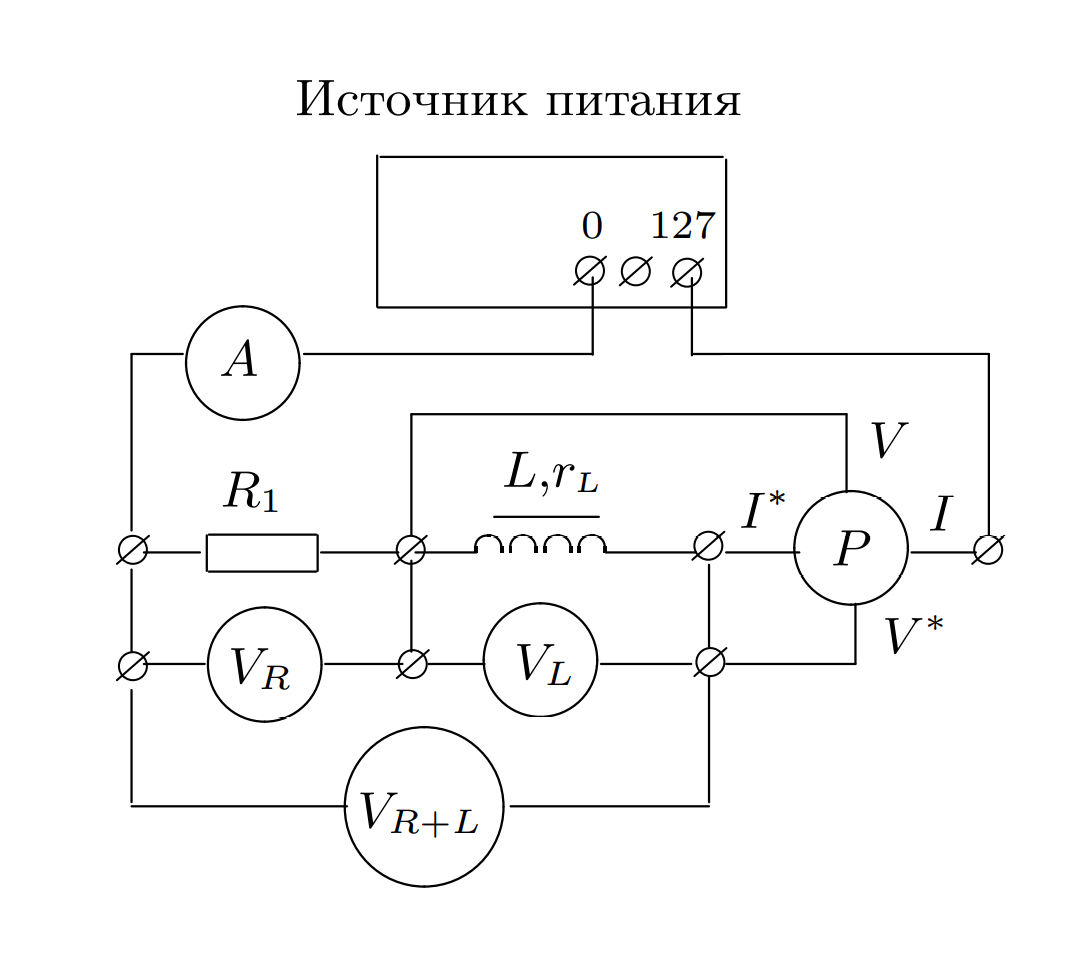
\includegraphics[scale=0.35]{img/Device.png}
            \caption{Схема экспериментальной установки} \label{Device}
        \end{figure}

        Ваттметр электродинамической системы состоит из двух катушек, одна из которых вращается в магнитном поле другой, если через них течёт ток. Токовая катушка ваттметра $II^*$ включается последовательно в исследуемую цепь, а катушка напряжений (потенциальная) $VV^*$ -- параллельно элементу, в котором измеряется выделяемая мощность.

        Схема установки для изучения резонанса напряжений изображена на рис. \ref{Device_2}. Последовательно соединены резистор $R_2\approx5~\Omega$, катушка $L$ и магазин ёмкостей $C$. Амперметр $A$ измеряет ток в цепи, вольтметр $V_C$ -- напряжение на ёмкости, вольтметр $V_{\Sigma}$ -- суммарное напряжение на контуре. Резонанс можно зафиксировать с помощью осциллографа, если подать на вход $X$ напряжение с контура, а на вход $Y$ -- напряжение с резистора $R_2$, пропорциональное току в цепи. В общем случае на экране виден эллипс. При резонансе эллипс вырождается в прямую линию.

        \begin{figure}[ht]
            \centering
            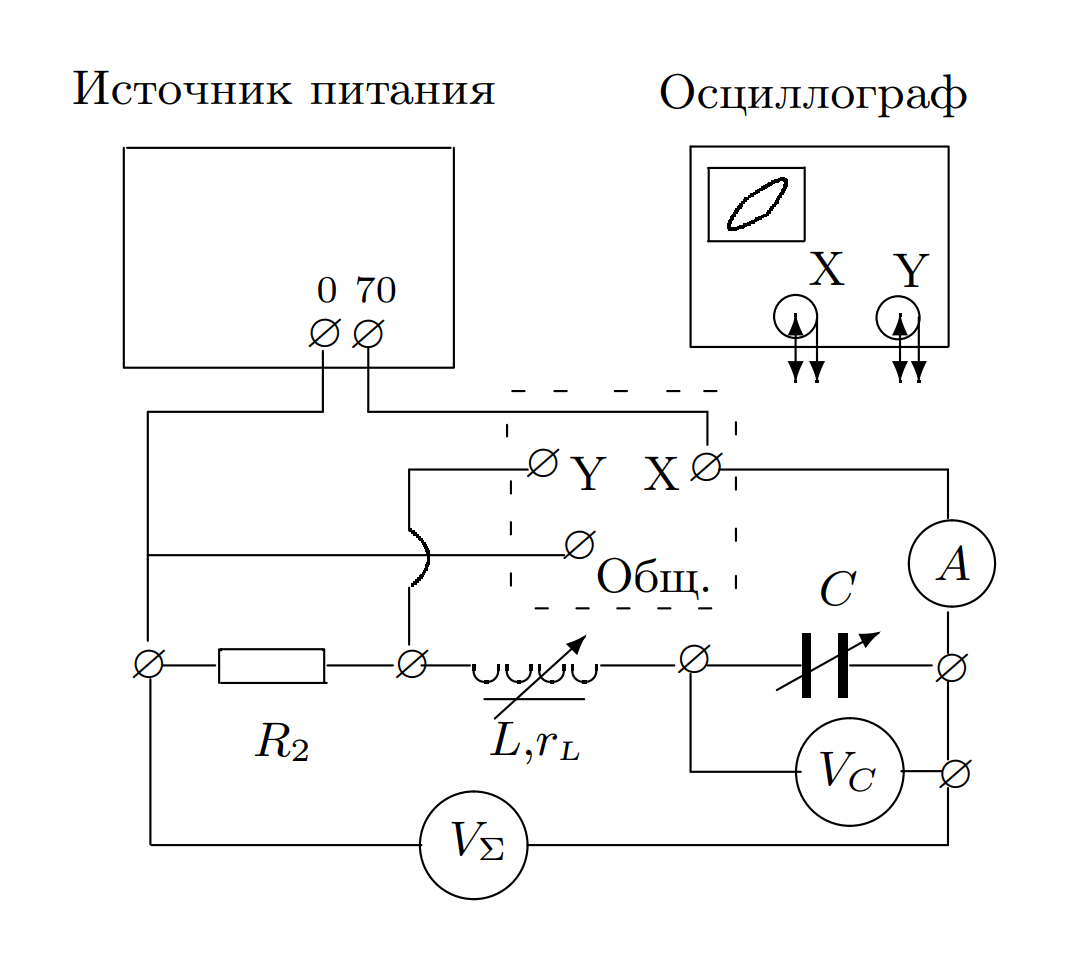
\includegraphics[scale=0.35]{img/Device_2.png}
            \caption{Схема экспериментальной установки} \label{Device_2}
        \end{figure}

        Резонансные напряжения на контуре $U_{\Sigma,\ \text{рез.}}$ и на ёмкости $U_{C,\ \text{рез.}}$ равны соответственно\[U_{\Sigma,\ \text{рез.}}=I_{\text{рез.}}R_{\Sigma},\ U_{C,\ \text{рез.}}=\frac{I_{\text{рез.}}}{\Omega C}.\]Отсюда\[Q=\frac{U_{C,\ \text{рез.}}}{U_{\Sigma,\ \text{рез.}}}.\]Это значит, что добротность контура может быть найдена по измеренным значениям напряжений на контуре и на конденсаторе при резонансе. Зная добротность контура и ёмкость $C$, можно рассчитать $R_{\Sigma}$, а затем определить $r_L$.

\end{document}
